\section{Observations \& Calculations}
	\subsection{GM characteristics}
		A gamma source $(Cs^{137})$ was used and the voltage was varied to get the data in \hyperref[tab:1]{Table 1}. From the data, the curve was plotted as shown in \hyperref[graph:1]{Figure 3}. Data was taken for 60s keeping the $Cs^{137}$ source at a distance of 6cm from the GM counter.

		\begin{table}[h]
	\centering
	\begin{tabular}{|c|c|c|c|}
	\hline
	\textbf{\begin{tabular}[c]{@{}c@{}}Angle\\ $(\theta)$\end{tabular}} & \textbf{Time (s)} & \textbf{Counts} & \textbf{\begin{tabular}[c]{@{}c@{}}Counts per\\ second $N(\theta)$\end{tabular}} \\ \hline
	\multirow{5}{*}{25} & \multirow{5}{*}{600} & 133 & \multirow{5}{*}{0.225} \\ \cline{3-3}
	 &  & 140 &  \\ \cline{3-3}
	 &  & 127 &  \\ \cline{3-3}
	 &  & 137 &  \\ \cline{3-3}
	 &  & 138 &  \\ \hline
	\multirow{5}{*}{20} & \multirow{5}{*}{200} & 164 & \multirow{5}{*}{0.940} \\ \cline{3-3}
	 &  & 198 &  \\ \cline{3-3}
	 &  & 186 &  \\ \cline{3-3}
	 &  & 195 &  \\ \cline{3-3}
	 &  & 197 &  \\ \hline
	\multirow{5}{*}{15} & \multirow{5}{*}{100} & 311 & \multirow{5}{*}{2.929} \\ \cline{3-3}
	 &  & 276 &  \\ \cline{3-3}
	 &  & 277 &  \\ \cline{3-3}
	 &  & 311 &  \\ \cline{3-3}
	 &  & 290 &  \\ \hline
	\multirow{5}{*}{10} & \multirow{5}{*}{100} & 1726 & \multirow{5}{*}{17.626} \\ \cline{3-3}
	 &  & 1811 &  \\ \cline{3-3}
	 &  & 1713 &  \\ \cline{3-3}
	 &  & 1754 &  \\ \cline{3-3}
	 &  & 1809 &  \\ \hline
	\multirow{5}{*}{5} & \multirow{5}{*}{100} & 2931 & \multirow{5}{*}{29.286} \\ \cline{3-3}
	 &  & 2938 &  \\ \cline{3-3}
	 &  & 2912 &  \\ \cline{3-3}
	 &  & 2931 &  \\ \cline{3-3}
	 &  & 2931 &  \\ \hline
	\multirow{5}{*}{-5} & \multirow{5}{*}{100} & 2934 & \multirow{5}{*}{29.343} \\ \cline{3-3}
	 &  & 2933 &  \\ \cline{3-3}
	 &  & 2935 &  \\ \cline{3-3}
	 &  & 2935 &  \\ \cline{3-3}
	 &  & 2935 &  \\ \hline
	\multirow{5}{*}{-10} & \multirow{5}{*}{100} & 1751 & \multirow{5}{*}{17.824} \\ \cline{3-3}
	 &  & 1778 &  \\ \cline{3-3}
	 &  & 1831 &  \\ \cline{3-3}
	 &  & 1787 &  \\ \cline{3-3}
	 &  & 1766 &  \\ \hline
	\multirow{5}{*}{-15} & \multirow{5}{*}{100} & 291 & \multirow{5}{*}{2.940} \\ \cline{3-3}
	 &  & 294 &  \\ \cline{3-3}
	 &  & 289 &  \\ \cline{3-3}
	 &  & 290 &  \\ \cline{3-3}
	 &  & 306 &  \\ \hline
	\multirow{5}{*}{-20} & \multirow{5}{*}{200} & 210 & \multirow{5}{*}{1.009} \\ \cline{3-3}
	 &  & 194 &  \\ \cline{3-3}
	 &  & 211 &  \\ \cline{3-3}
	 &  & 201 &  \\ \cline{3-3}
	 &  & 194 &  \\ \hline
	\multirow{5}{*}{-25} & \multirow{5}{*}{600} & 133 & \multirow{5}{*}{0.225} \\ \cline{3-3}
	 &  & 140 &  \\ \cline{3-3}
	 &  & 127 &  \\ \cline{3-3}
	 &  & 135 &  \\ \cline{3-3}
	 &  & 141 &  \\ \hline
	\end{tabular}
	\caption{Table for $N(\theta)$ for 5mm thick Gold foil}
	\label{tab:1}
\end{table}
		\begin{figure}[h]
			\centering
			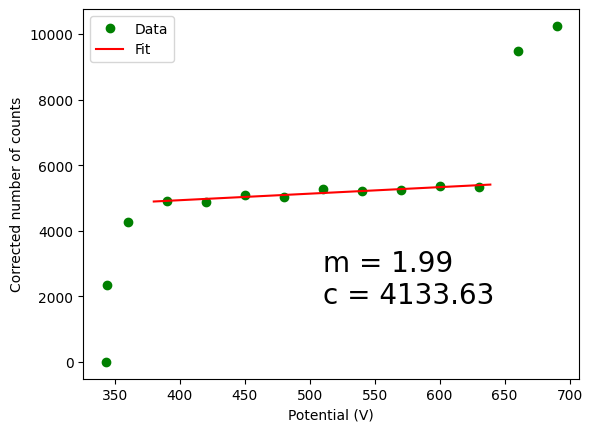
\includegraphics[width=0.9\columnwidth]{images/g1.png}
			\caption{Graph of GM characteristics}
			\label{graph:1}
		\end{figure}

		From the graph we can see:
		\begin{enumerate}
			\item Lower threshol volatge = $390 V$
			\item Upper threshold voltage = $630 V$
			\item Plateu length = $(630 - 390) V = 240 V$
			\item Counts at lower threshold voltage = $(N) = 4910$
			\item Slope = $1.99$
			\item Plateau Slope percent $(s) = \frac{slope}{N}*10000 = \frac{1.99}{4910}*10000 = 4.073\%$
			\item Operating Volatage = $\frac{600+360}{2} = 510 V$
		\end{enumerate}

	\subsection{Inverse Square Law}
		\begin{table}[H]
    \centering
    \begin{tabular}{|c|c|c|c|}
        \hline
        $V_{DC}$ & $V_{DUT}$ & $V_{OUT}$ & $C_{DUT}$   \\ \hline
        0        & 0.074     & 0.459     & 127.837 \\
        0.1      & 0.109     & 0.451     &  85.276 \\
        0.2      & 0.232     & 0.447     &  39.709 \\
        0.3      & 0.299     & 0.438     &  30.191 \\
        0.4      & 0.389     & 0.432     &  22.888 \\
        0.5      & 0.463     & 0.432     &  19.230 \\
        0.6      & 0.564     & 0.426     &  15.567 \\
        0.7      & 0.662     & 0.420     &  13.075 \\
        0.8      & 0.760     & 0.435     &  11.796 \\
        0.9      & 0.846     & 0.430     &  10.475 \\
        1        & 0.941     & 0.426     &   9.330 \\
        1.1      & 1.058     & 0.427     &   8.318 \\
        1.2      & 1.174     & 0.422     &   7.408 \\
        1.3      & 1.267     & 0.418     &   6.799 \\
        1.4      & 1.357     & 0.416     &   6.318 \\
        1.5      & 1.464     & 0.412     &   5.800 \\
        1.6      & 1.559     & 0.409     &   5.406 \\ \hline
    \end{tabular}
    \caption{Data for light condition}
    \label{tab:2}
\end{table}
		\begin{table}[]
	\centering
	\begin{tabular}{|l|l|}
	\hline
		H(gauss) & V(mV) \\ \hline
		2390 & -0.061 \\ \hline
		2540 & -0.062 \\ \hline
		3160 & -0.063 \\ \hline
		3480 & -0.064 \\ \hline
		4200 & -0.065 \\ \hline
		4500 & -0.066 \\ \hline
		4780 & -0.067 \\ \hline
		5200 & -0.068 \\ \hline
		5180 & -0.069 \\ \hline
	\end{tabular}
	\caption{Magnetoresistance Data for $I=101.0mA$}
	\label{tab:mag2}
\end{table}
		
		\begin{figure}[h]
			\centering
			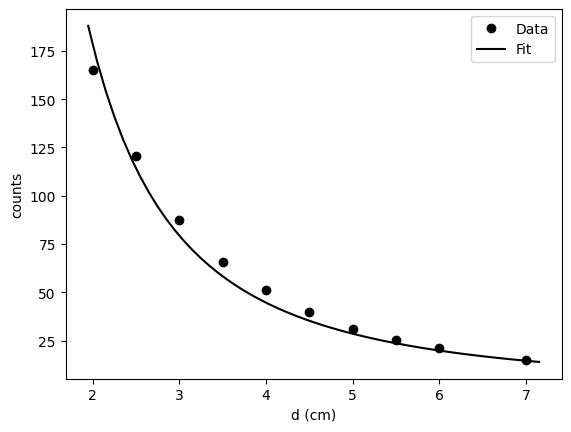
\includegraphics[width=\columnwidth]{images/g3.png}
			\caption{Counts vs distance graph}
			\label{graph:3}
		\end{figure}

		We can clearly see in \hyperref{tab:3}{Table 3} that the value of $Rd^2$ is almost constant. Thus, we can say that the inverse square law is valid for the given data.
		
		\begin{figure}[h]
			\centering
			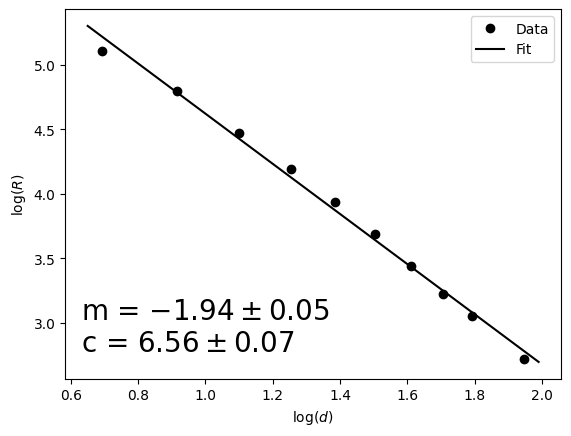
\includegraphics[width=\columnwidth]{images/g2.png}
			\caption{$\log(d)$ vs $\log(R)$ graph}
			\label{graph:2}
		\end{figure}

		From the graph in \hyperref[graph:2]{Figure 4}, we can see that the data points lie on a straight line. Also the slope of the line is $-2$. Thus, we can say that the inverse square law is valid for the given data.


		\begin{table}[h]
	\centering
	\resizebox{\columnwidth}{!}{%
		\begin{tabular}{|c|c|c|c|c|c|}
			\hline
			\textbf{Source}                      & \textbf{Distance (cm)} & \textbf{Counts} & \textbf{Corrected Counts} & \textbf{Average}         & \multicolumn{1}{l|}{\textbf{CPS}} \\ \hline
			\multirow{3}{*}{\textbf{$Cs^{137}$}} & \multirow{3}{*}{10}    & 738             & 655                       & \multirow{3}{*}{670.667} & \multirow{3}{*}{11.178}           \\ \cline{3-4}
			                                     &                        & 766             & 683                       &                          &                                   \\ \cline{3-4}
			                                     &                        & 757             & 674                       &                          &                                   \\ \hline
			\multirow{3}{*}{\textbf{$Tl^{204}$}} & \multirow{3}{*}{2}     & 2306            & 2223                      & \multirow{3}{*}{2224}    & \multirow{3}{*}{37.067}           \\ \cline{3-4}
			                                     &                        & 2309            & 2226                      &                          &                                   \\ \cline{3-4}
			                                     &                        & 2306            & 2223                      &                          &                                   \\ \hline
		\end{tabular}%
	}
	\caption{Efficiency Data}
	\label{tab:4}
\end{table}  % This table belongs to Efficiency section
	\subsection{Efficiency}
		Given data:
		\begin{itemize}
			\item $d = 1.5cm$
			\item Activity of $Cs^{137}$ = $86 kBq$ (as of May 2016)
			\item Activity of $Tl^{204}$ = $10 kBq$ (as of May 2016)
			\item $\therefore$ Activity of $Cs^{137} \approx 73447 Bq$ (half life $\approx$ 30 years) (after 6 years 11 months, in March 2023)
			\item $\therefore$ Activity of $Tl^{204} \approx  2847 Bq$ (half life $\approx$ 3.77 years) (after 6 years 11 months, in March 2023)
		\end{itemize}

		Therefore using \hyperref[eq:2]{Equation 2} we get:
		\begin{itemize}
			\item $DPS_{Cs} = \frac{73447 \times (1.5)^2}{1600} = 351.56$
			\item $DPS_{Tl} = \frac{2847 \times (1.5)^2}{1600} = 120.94$
		\end{itemize}

		From \hyperref[tab:4]{Table 4}, we can see that:
		\begin{itemize}
			\item $CPS_{Cs} = 11.178$
			\item $CPS_{Tl} =  37.067$
		\end{itemize}

		Thus calculating the efficiency using \hyperref[eq:1]{Equation 1}
		\begin{itemize}
			\item Eff$_{Cs} = \frac{CPS_{Cs}}{DPS_{Cs}}*100 = \frac{11.178}{351.56}*100 = 31.62\%$
			\item Eff$_{Tl} = \frac{CPS_{Tl}}{DPS_{Tl}}*100 = \frac{37.067}{120.94}*100 = 30.65\%$
		\end{itemize}

		We can see that for both the sources, the efficiency is almost the same. Thus, we can say that the efficiency is independent of the source and is a property of the detector.
		
		\begin{figure}[h]
			\centering
			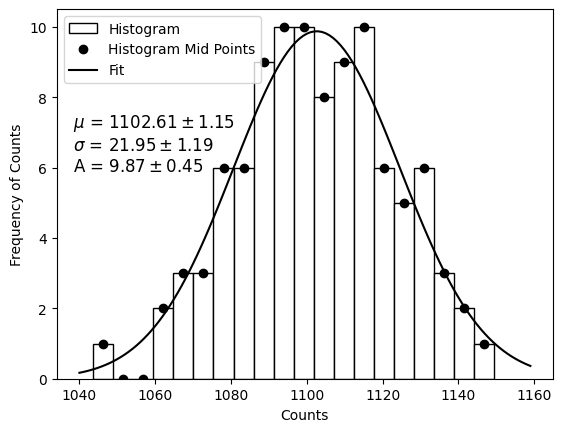
\includegraphics[width=\columnwidth]{images/g4.png}
			\caption{Counts vs frequency graph}
			\label{graph:4}
		\end{figure}

	\subsection{Counting Statistics}

		For the counting statistics, we took 100 counts with the $Cs^{137}$ source. By plotting the counts vs their frequencies of occurence, we plotted \hyperref[graph:4]{Figure 6}. Although here the data (which is only 100 numbers) is not tabulated, you can easily see the whole data if you get this excel sheet: \href{https://github.com/PeithonKing/lab\_reports/raw/main/Sem6/Nuclear\_Physics/Expt1/gm1.xlsx}{https://github.com/PeithonKing/lab\_reports/raw/main/
		Sem6/Nuclear\_Physics/Expt1/gm1.xlsx}.
		
		From the graph, we see that the data is mostly concentrated around the mean value. Thus, we can say that the data is normally distributed.
